%
% this file is encoded in utf-8
% v1.7
% do not change the content of this file
% unless the thesis layout rule is changed
% 無須修改本檔內容，除非校方修改了
% 封面、書名頁、中文摘要、英文摘要、誌謝、目錄、表目錄、圖目錄、符號說明
% 等頁之格式
% this file is encoded in utf-8
%v1.7

% make the line spacing in effect
\renewcommand{\baselinestretch}{\mybaselinestretch}
\large % it needs a font size changing command to be effective

 % user's names; to replace those default variable definitions
%
% this file is encoded in utf-8
% v1.7

% 論文題目 (中文)
\newcommand\cTitle{
    具情節記憶之高效輕量視覺語言模型應用於資源受限邊緣裝置部署
}

% 論文題目 (英文)
\newcommand\eTitle{
    Efficient Tiny Vision-Language Models with Episodic Memory for Resource-Constrained Edge Deployment
}

% 我的姓名 (中文)
\newcommand\myCname{Euhid~Aman}

% 我的姓名 (英文)
\newcommand\myEname{Euhid~Aman}

% 我的學號
\newcommand\myStudentID{M11315803}

% 指導教授A的姓名 (中文)
\newcommand\advisorCnameA{鮑興國~博士}

% 指導教授A的姓名 (英文)
\newcommand\advisorEnameA{Prof.~Hsing-Kuo~Pao}

% 指導教授B的姓名 (中文)
\newcommand\advisorCnameB{}

% 指導教授B的姓名 (英文)
\newcommand\advisorEnameB{}

% 指導教授C的姓名 (中文)
\newcommand\advisorCnameC{}

% 指導教授C的姓名 (英文)
\newcommand\advisorEnameC{}

% 校名 (中文)
\newcommand\univCname{國立台灣科技大學}

% 系所名 (中文)
\newcommand\deptCname{資訊工程系}

% 學位名 (中文)
\newcommand\degreeCname{碩士}

% 口試年份 (中文、民國)
\newcommand\cYear{一一四}

% 口試月份 (中文)
\newcommand\cMonth{七}

% 口試日 (中文)
\newcommand\cDay{一}

%畢業級別；用於書背列印；若無此需要可忽略
\newcommand\GraduationClass{114}

\newcommand\itsempty{}
%%%%%%%%%%%%%%%%%%%%%%%%%%%%%%%
%       ntust cover 封面
%%%%%%%%%%%%%%%%%%%%%%%%%%%%%%%
%
\begin{titlepage}
% no page number
% next page will be page 1

% aligned to the center of the page
\begin{center}
% font size (relative to 12 pt):
% \large (14pt) < \Large (18pt) < \LARGE (20pt) < \huge (24pt)< \Huge (24 pt)
%



\begin{figure}[htbp]
	% \begin{minipage}[b]{5cm} 
	\begin{minipage}[b]{.2\textwidth} 
		\centering
            \vfill
		
\includegraphics[width=1.1in]{matters/front/ntust_logo.eps}
		\label{fig:ntust_logo}
	\end{minipage}% 
	\begin{minipage}[b]{.8\textwidth} 
	\centering
	\makebox[\linewidth][c]{\Huge{\univCname}}\\  %顯示中文校名
	\vspace{0.5cm}
	\makebox[.6\linewidth][s]{\Huge{\deptCname}}\\ %顯示中文系所名
	\vspace{0.5cm}
	\end{minipage}%
\\ 
\rule{\textwidth}{3pt}
\end{figure}
%\hfill


\vspace{1cm}
\makebox[0.5\textwidth][s]{\textbf{\Huge{\degreeCname 學位論文}}}\\ %顯示論文種類 (中文)
\vspace{1cm}
%
% Set the line spacing to single for the titles (to compress the lines)
\renewcommand{\baselinestretch}{1}   %行距 1 倍
%\large % it needs a font size changing command to be effective
\Large{\cTitle}\\  % 中文題目
%
\vspace{1cm}
%
\Large{\eTitle}\\ %英文題目
% \vspace{5em}
\vfill
\begin{tabular}{r@{}l}
    \makebox[.25\linewidth][s]{\Large{研究生：}} & \Large{\myCname}  % 顯示作者中文名
    \\ [.3em]
    %
    \makebox[.25\linewidth][s]{\Large{學號：}} & \Large{\myStudentID}  %顯示指導教授A中文名
    \\[1em]
    %
    \makebox[.25\linewidth][s]{\Large{指導教授：}} & \Large{\advisorCnameA}  %顯示指導教授A中文名
    \\
    \ifthenelse{\equal{\advisorCnameB}{}} % 判斷是否有共同指導的教授 B
        {}
        {\makebox[.25\linewidth][s]{} & \Large{\advisorCnameB}\\} % 共同指導的教授 B
    \ifthenelse{\equal{\advisorCnameC}{}} % 判斷是否有共同指導的教授 C
        {}
        {\makebox[.25\linewidth][s]{} & \Large{\advisorCnameC}\\} % 共同指導的教授 C
    
\end{tabular}

\makebox[.8\textwidth][s]{\Large{中華民國{\cYear}年{\cMonth}月{\cDay}日}}%
%
\end{center}
% Resume the line spacing to the desired setting
\renewcommand{\baselinestretch}{\mybaselinestretch}   %恢復原設定
% it needs a font size changing command to be effective
% restore the font size to normal
\normalsize
\end{titlepage}

%% 從摘要到本文之前的部份以小寫羅馬數字印頁碼
% 但是從「書名頁」(但不印頁碼) 就開始計算
\setcounter{page}{1}
\pagenumbering{Roman}
%%%%%%%%%%%%%%%%%%%%%%%%%%%%%%%%%%%%%%%%%%%%%%%%%%%%%%%%%%
%       指導教授推薦書 Recommendation Form
%%%%%%%%%%%%%%%%%%%%%%%%%%%%%%%%%%%%%%%%%%%%%%%%%%%%%%%%%%
%
% insert the printed standard form when the thesis is ready to bind
% 在口試完成後，再將已簽名的推薦書放入以便裝訂
% create an entry in table of contents for 推薦書
% 目前送出空白頁
% \newpage{\thispagestyle{empty}\addcontentsline{toc}{chapter}{\nameInnerCover}\mbox{}\clearpage}
\addcontentsline{toc}{chapter}{\nameInnerCover}

\includepdf[pages=-]{000_frontpages/01_recommendation_form.pdf}
%\newpage

% 判斷是否要浮水印？
\ifx\mywatermark\undefined 
  \thispagestyle{empty}  % 無頁碼、無 header (無浮水印)
\else
  \thispagestyle{EmptyWaterMarkPage} % 無頁碼、有浮水印
\fi

%%%%%%%%%%%%%%%%%%%%%%%%%%%%%%%%%%%%%%%%%%%%%%%%%%%%%%%%%%
%       論文口試委員審定書 Qualification Form
%%%%%%%%%%%%%%%%%%%%%%%%%%%%%%%%%%%%%%%%%%%%%%%%%%%%%%%%%%
%
% insert the printed standard form when the thesis is ready to bind
% 在口試完成後，再將已簽名的審定書放入以便裝訂
% create an entry in table of contents for 審定書
% 目前送出空白頁
% \newpage{\thispagestyle{empty}\addcontentsline{toc}{chapter}{\nameCommitteeForm}\mbox{}\clearpage}
\addcontentsline{toc}{chapter}{\nameCommitteeForm}
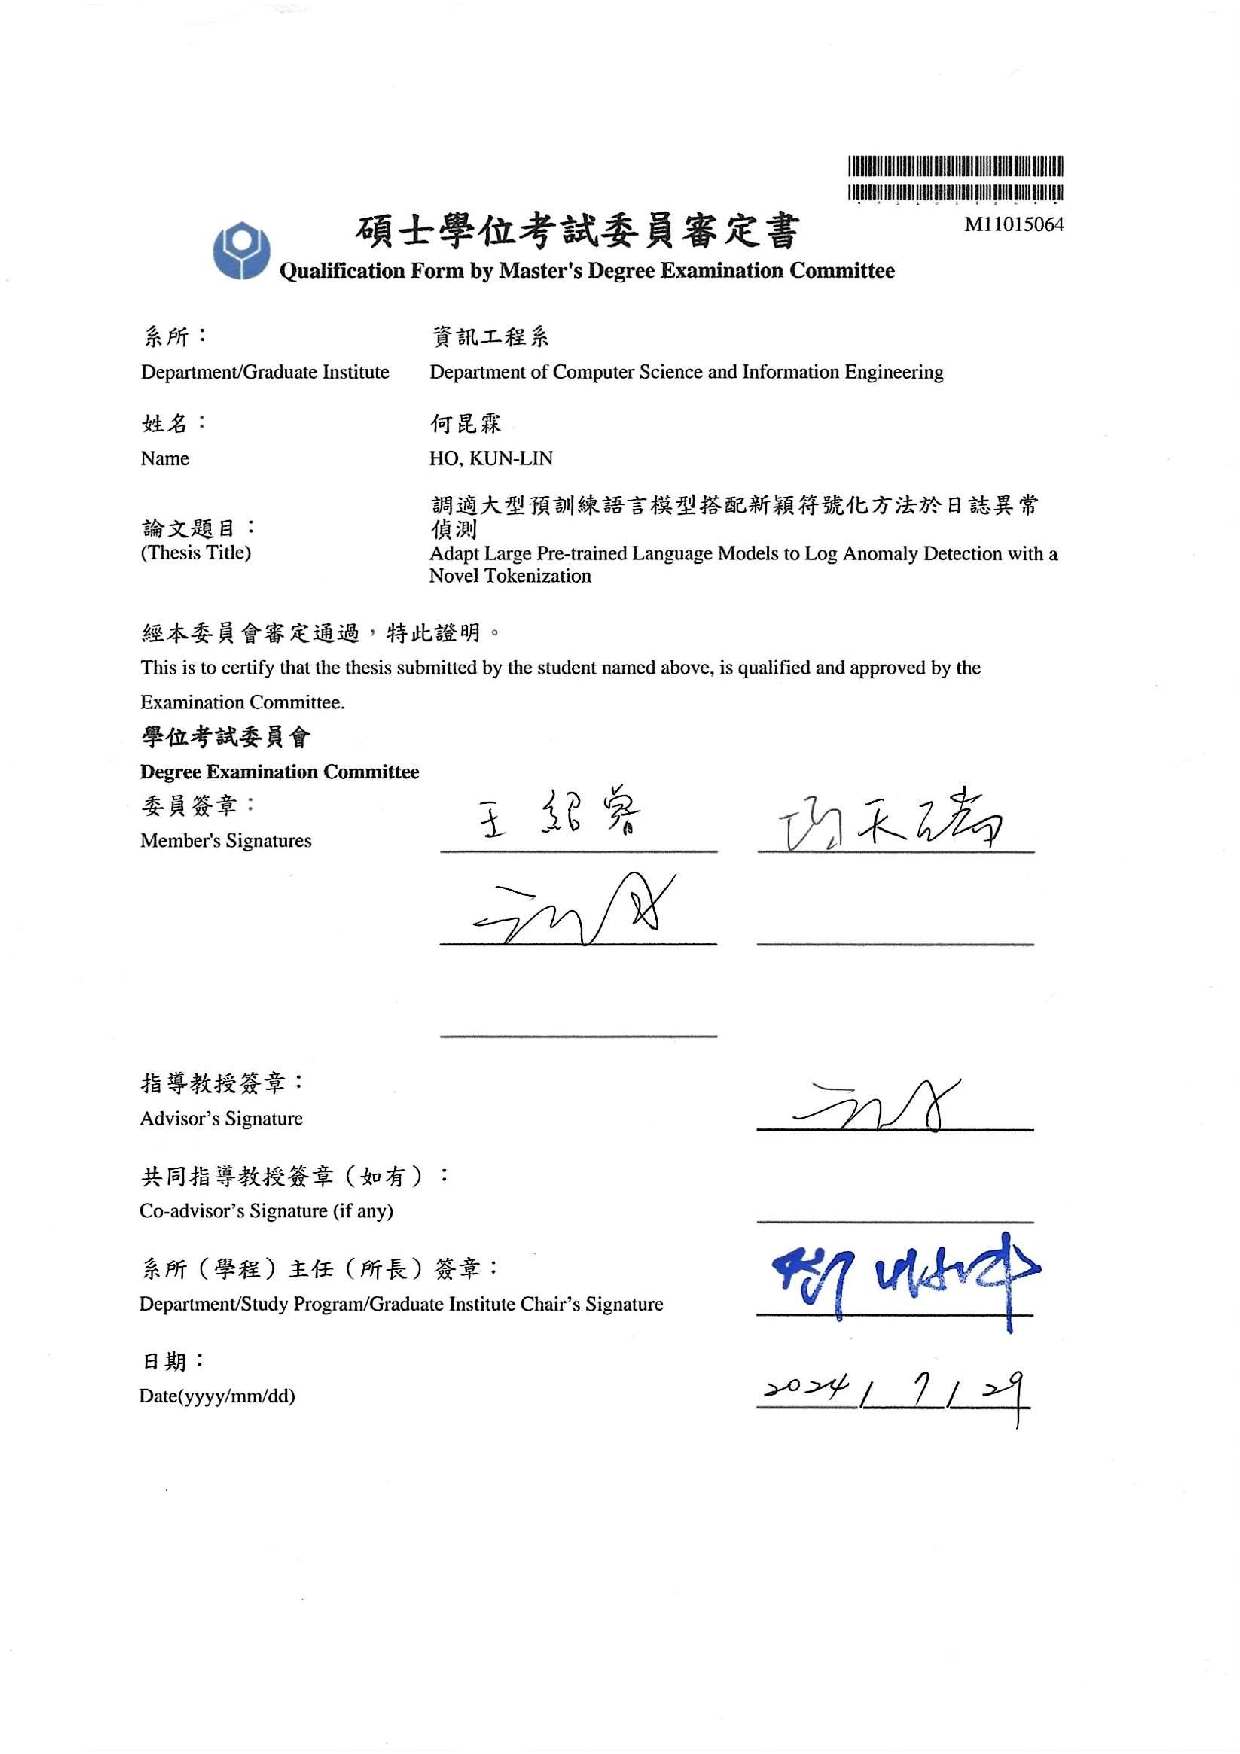
\includepdf[pages=-]{000_frontpages/02_qualification_form.pdf}


%%%%%%%%%%%%%%%%%%%%%%%%%%%%%%%%%%%%%%%%%%%%%%%%%%%%%%%%%%
%              中文摘要 Chinese Abstract
%%%%%%%%%%%%%%%%%%%%%%%%%%%%%%%%%%%%%%%%%%%%%%%%%%%%%%%%%%

\newpage
\thispagestyle{plain}  % 無 header，但在浮水印模式下會有浮水印
% create an entry in table of contents for 中文摘要
\addcontentsline{toc}{chapter}{\nameCabstract}

% aligned to the center of the page
\begin{center}
% font size (relative to 12 pt):
% \large (14pt) < \Large (18pt) < \LARGE (20pt) < \huge (24pt)< \Huge (24 pt)
% Set the line spacing to single for the names (to compress the lines)
\renewcommand{\baselinestretch}{1}   %行距 1 倍
% it needs a font size changing command to be effective
\makebox[.2\linewidth][s]{\Large{摘要}}\\
\end{center}
% Resume the line spacing to the desired setting
\renewcommand{\baselinestretch}{\mybaselinestretch}   %恢復原設定
%it needs a font size changing command to be effective
% restore the font size to normal
\normalsize
%%%%%%%%%%%%%
{\renewcommand{\baselinestretch}{1.2}\normalsize
大型視覺語言模型（Vision-Language Models，VLMs）在多模態任務上表現卓越，但高度依賴雲端基礎設施與高效能 GPU，難以直接部署於資源受限的邊緣環境。本論文針對記憶體低於 800 MB、純 CPU 推理、延遲低於 10 毫秒及任務關鍵場景零幻覺容忍等嚴苛約束，開發適用於裝置端部署的輕量視覺語言模型。

本論文提出兩套系統。\textbf{BitMar} 為 1400 萬參數、採用 1.58 位元三元量化的多模態模型，整合跨模態融合管線與外部情節記憶矩陣（512 槽位，128 維）。啟用情節記憶後，推理吞吐量提升約 7.5 倍，能耗降低 79\%，並在實體追蹤、組合推理及視覺問答任務上獲得 3 至 4 個百分點的準確率提升，驗證了極限量化、跨模態融合與情節記憶在同一架構中共存的可行性。\textbf{EmberVLM} 為本論文主要貢獻，總計 1.64 億參數（4000 萬可訓練），採用四階段課程式訓練策略。其情節記憶模組採用高斯距離定址與新穎性觸發動態寫入機制，每步推理僅增加 1.2 MB 記憶體佔用及不足 3\% 的浮點運算量，可將機器人選擇任務之巨集 F1 分數從 0.035 提升至 0.297。其視覺缺失精煉器（VA Refiner）為免訓練的幻覺抑制機制，透過雙視角邏輯差異分析與解碼器中間層神經元激活監控，無需額外前向傳遞即可抑制視覺上無依據的輸出。

EmberVLM 在三項任務關鍵基準上取得最佳成績：Top-N 機器人選擇（巨集 F1 = 0.42）、緊急視覺辨識（準確率 0.64）及地理災害理解（準確率 0.72）。完整推理堆疊在純 CPU 裝置上僅需 5.22 毫秒，記憶體佔用低於 800 MB。VA 精煉器將對抗性幻覺率從 29\% 降至 22\%。全訓練週期碳排放實測為 25.3 kg CO$_2$eq，展示了任務關鍵邊緣人工智慧的永續訓練路徑。

\chinesekeywords{邊緣人工智慧、視覺語言模型、情節記憶、幻覺抑制、模型量化、資源受限部署}
}


%%%%%%%%%%%%%%%%%%%%%%%%%%%%%%%%%%%%%%%%%%%%%%%%%%%%%%%%%%
%              英文摘要 English Abstract
%%%%%%%%%%%%%%%%%%%%%%%%%%%%%%%%%%%%%%%%%%%%%%%%%%%%%%%%%%

\newpage
%\thispagestyle{plain}  % 無 header，但在浮水印模式下會有浮水印
\chapter*{\protect\makebox{Abstract}}
% create an entry in table of contents for 英文摘要
\addcontentsline{toc}{chapter}{\nameEabstract}

{\renewcommand{\baselinestretch}{1.2}\normalsize
Large vision-language models (VLMs) achieve strong multimodal performance but depend entirely on cloud infrastructure and high-end GPU hardware, making them unsuitable for resource-constrained, offline, and privacy-sensitive deployment scenarios. This thesis develops compact VLMs for on-device inference under simultaneous hard constraints: under 800~MB RAM, CPU-only execution, sub-10~ms latency, and zero tolerance for hallucinated outputs in mission-critical settings.

Two systems are presented. \textbf{BitMar} is a 14M-parameter, 1.58-bit ternary-quantized multimodal model integrating a cross-modal fusion pipeline with an external episodic memory matrix (512 slots, 128 dimensions). Enabling episodic memory yields approximately $7.5\times$ throughput improvement and 79\% energy reduction over the memory-free baseline, alongside 3--4 percentage-point accuracy gains on entity tracking, compositional reasoning, and visual question answering. BitMar establishes the foundational compatibility of extreme quantization, cross-modal fusion, and episodic memory in a single architecture. \textbf{EmberVLM} is the primary contribution: a 164M-parameter VLM (40M trainable) with a four-stage training curriculum. Its Episodic Memory Module employs Gaussian distance-based addressing and novelty-triggered online writes, adding only 1.2~MB RAM and under 3\% extra FLOPs per inference step, boosting robot-selection Macro-F1 from 0.035 to 0.297. Its Visual Absence (VA) Refiner is a training-free hallucination control mechanism fusing logit-space dual-view consistency with neuron-level mid-decoder activation monitoring, requiring no additional forward passes.

EmberVLM achieves the best reported results among sub-billion-parameter models on three mission-critical benchmarks: Top-N Robot Selection (Macro-F1~=~0.42), emergency visual recognition (Accuracy~=~0.64), and geospatial disaster understanding (Accuracy~=~0.72). The full inference stack runs at 5.22~ms per sample on a CPU-only device with under 800~MB RAM. The VA Refiner reduces adversarial hallucination rate from 29\% to 22\%. Total measured training emissions are 25.3~kg~CO$_2$eq, demonstrating that mission-critical multimodal AI can be trained sustainably.

\keywords{Edge AI, Vision-Language Models, Episodic Memory, Hallucination Mitigation, Model Quantization, Resource-Constrained Deployment}
}


%%%%%%%%%%%%%%%%%%%%%%%%%%%%%%%%%%%%%%%%%%%%%%%%%%%%%%%%%%
%                誌謝 Acknowledgements
%%%%%%%%%%%%%%%%%%%%%%%%%%%%%%%%%%%%%%%%%%%%%%%%%%%%%%%%%%
%
% Acknowledgment
\newpage
\chapter*{\protect\makebox{\nameAckn}} %\makebox{} is fragile; need protect
\addcontentsline{toc}{chapter}{\nameAckn}
% TODO: Student to fill in acknowledgements



%%%%%%%%%%%%%%%%%%%%%%%%%%%%%%%%%%%%%%%%%%%%%%%%%%%%%%%%%%
%         目錄 Table of Contents (auto generated)
%%%%%%%%%%%%%%%%%%%%%%%%%%%%%%%%%%%%%%%%%%%%%%%%%%%%%%%%%%
%
% Table of contents
\newpage
\renewcommand{\contentsname}{\protect\makebox{\nameToc}}
%\makebox{} is fragile; need protect
\addcontentsline{toc}{chapter}{\nameToc}
\tableofcontents

%%%%%%%%%%%%%%%%%%%%%%%%%%%%%%%
%       圖目錄 
%%%%%%%%%%%%%%%%%%%%%%%%%%%%%%%
%
% List of Figures
\newpage
\renewcommand{\listfigurename}{\protect\makebox{\nameTof}}
%\makebox{} is fragile; need protect
\addcontentsline{toc}{chapter}{\nameTof}
\listoffigures

%%%%%%%%%%%%%%%%%%%%%%%%%%%%%%%
%       表目錄 
%%%%%%%%%%%%%%%%%%%%%%%%%%%%%%%
%
% List of Tables
\newpage
\renewcommand{\listtablename}{\protect\makebox{\nameLot}}
%\makebox{} is fragile; need protect
\addcontentsline{toc}{chapter}{\nameLot}
\listoftables

%%%%%%%%%%%%%%%%%%%%%%%%%%%%%%%
%       演算法目錄 
%%%%%%%%%%%%%%%%%%%%%%%%%%%%%%%
%
% List of Figures
\newpage
\renewcommand{\listalgorithmname}{\protect\makebox{\nameToa}}
%\makebox{} is fragile; need protect
\addcontentsline{toc}{chapter}{\nameToa}
\listofalgorithms

\newpage
%% 論文本體頁碼回復為阿拉伯數字計頁，並從頭起算
\pagenumbering{arabic}
%%%%%%%%%%%%%%%%%%%%%%%%%%%%%%%%